\section{Tablas y tabulación}

Para trabajar con tablas, se tiene que usar los comandos \textbf{\textbackslash{begin}} y \textbf{\textbackslash{end}}, seguido de \textbf{table}: es un indicativo para señalar que se comenzará a trabajar con una tabla, y el comando \textbf{tabular} (que tiene el mismo inicio de comando \textit{begin} y \textit{end}) es propiamente la tabla.

El comando \textbf{\textbackslash{caption\{\}}} dentro de \textbf{table}, es usado para darle un título a la tabla y el comando \textbf{label} funciona para referenciar la tabla en un texto o la sección de referencias.
\begin{lstlisting}
    \begin{table}
        \caption{Nombre}
        \label{tab: n}
        \begin{tabular}
             &  \\
             & 
        \end{tabular}
    \end{table}
\end{lstlisting}

Al trabajar con \textit{tabular}, abrimos un par de llaves para ingresar parámetros que indican la alineación del contenido de cada columna (si la tabla tiene tres columnas, cada una puede tener distinta alineación). Por defecto, la tabla no tiene líneas verticales de separación de columnas, estas pueden ser agregadas en dentro de estos parámetros con una línea vertical \textbf{\(|\)} entre cada parámetro de alineación; para agregar líneas horizontales de separación de filas a la tabla, se usa el comando \textbf{\textbackslash{hline}}.

La Tabla \ref{tab: 1} solamente trata la estructura básica de una tabla, sin líneas verticales ni horizontales, mientras que la Tabla \ref{tab: 2} involucra otra alineación de columnas y todos sus bordes:
\begin{lstlisting}
    \begin{table}[H]
        \begin{center}
            \caption{Ejemplo estructura básica de una tabla}
            \label{tab: 1}
            \begin{tabular}{l c r }
                C1 & C2 & C3 \\
                C4 & C5 & C6 
            \end{tabular}
        \end{center}
    \end{table}
    
    \begin{table}[H]
        \begin{center}
            \caption{Ejemplo \textbackslash{hline} y barras verticales}
            \label{tab: 2}
            \begin{tabular}{|c|c|c|}
                \hline
                C1 & C2 & C3 \\
                \hline
                C4 & C5 & C6 \\
                 \hline
            \end{tabular}
        \end{center}
    \end{table}
\end{lstlisting}
\begin{table}[H]
    \begin{center}
        \caption{Ejemplo estructura básica de una tabla}
        \label{tab: 1}
        \begin{tabular}{l c r }
            C1 & C2 & C3 \\
            C4 & C5 & C6 
        \end{tabular}
    \end{center}
\end{table}

\begin{table}[H]
    \begin{center}
        \caption{Ejemplo \textbackslash{hline} y barras verticales}
        \label{tab: 2}
        \begin{tabular}{|c|c|c|}
            \hline
            C1 & C2 & C3 \\
            \hline
            C4 & C5 & C6 \\
             \hline
        \end{tabular}
    \end{center}
\end{table}

Si pone atención, se dará cuenta que las dos diagonales invertidas (\textbackslash\textbackslash) funcionan para pasar entre fila y fila dentro de una tabla, pero, ¿y si yo quiero dar saltos de línea dentro de una celda?, recordemos que esas mismas diagonales son necesarias para dar un salto en los párrafos.

Podemos incluir el comando anteriormente mencionado: \textbackslash{parbox\{\}\{\}} dentro de las celdas para poder dar saltos de línea tranquilamente (\textit{Tabla \ref{tab: 3}}):
\begin{lstlisting}
    \begin{table}[H]
        \begin{center}
            \caption{Ejemplo \textbackslash{hline} y barras verticales}
            \label{tab: 3}
            \begin{tabular}{|c|c|c|}
                \hline
                C1 & C2 & \parbox{3cm}{C3.1 \\ C3.2 \\ C3.3} \\
                \hline
                C4 & C5 & \parbox{3cm}{C6.1 \\ C6.2 \\ C6.3} \\
                 \hline
            \end{tabular}
        \end{center}
    \end{table}
\end{lstlisting}
\begin{table}[H]
    \begin{center}
        \caption{Ejemplo \textbackslash{hline} y barras verticales}
        \label{tab: 3}
        \begin{tabular}{|c|c|c|}
            \hline
            C1 & C2 & \parbox{3cm}{C3.1 \\ C3.2 \\ C3.3} \\
            \hline
            C4 & C5 & \parbox{3cm}{C6.1 \\ C6.2 \\ C6.3} \\
            \hline
        \end{tabular}
    \end{center}
\end{table}


\subsection{Ubicación inicial y posicionamiento}

Las tablas suelen ser ubicadas del lado izquierdo cuando son insertadas, podemos usar los comandos \textbf{\textbackslash{begin\{center\}}} y \textbf{\textbackslash{end\{center\}}} o \textbf{\textbackslash{centering}} para centrarlas en el documento, personalmente recomiendo \textit{center} porque es más fácil de controlar.
\begin{lstlisting}
    \begin{center}
        texto
    \end{center}
    
    \centering
\end{lstlisting}

El posicionamiento de tablas en el texto del documento es otro punto a considerar, esto aplica para tablas, ecuaciones y figuras, pero lo trataremos específicamente para tablas.

En un editor de texto, como sería Word, insertamos una tabla en la posición actual del cursor, esto puede ser al inicio o final del documento, o después de un párrafo, y la tabla se posicionaría en el documento según cómo se mueva el párrafo, imagen u otro objeto previo a la tabla.

\LaTeX por otra parte, pone las tablas en la parte superior de la página donde quedó el último párrafo, imagen, figura u objeto por defecto, esto puede ocasionar problemas si un texto que referencia a la tabla queda en una página distinta o no convence el posicionamiento de la tabla con respecto al contenido del documento. El vistazo a lo que nos referimos se encuentra en las \textit{Figuras \ref{fig: 2}} y \textit{\ref{fig: 3}}:
\begin{figure}[H]
    \begin{center}
        \caption{Mal posicionamiento de tablas, figuras u otros objetos 1}
        \label{fig: 2}
        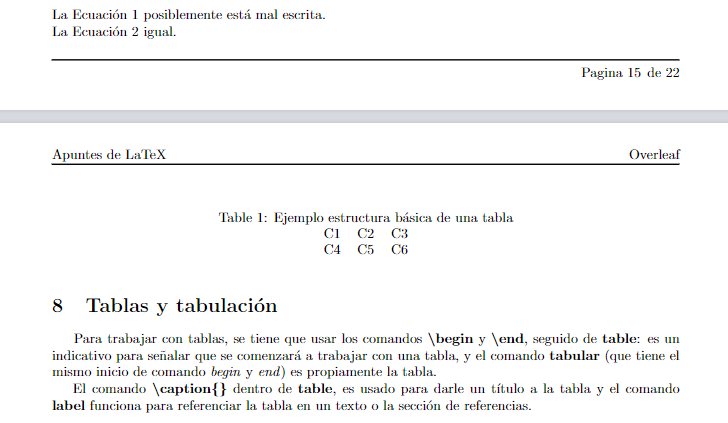
\includegraphics[width=\textwidth]{recursos/tablas_mal pos_1.png}
    \end{center}
\end{figure}
\begin{figure}[H]
    \begin{center}
        \caption{Mal posicionamiento de tablas, figuras u otros objetos 2}
        \label{fig: 3}
        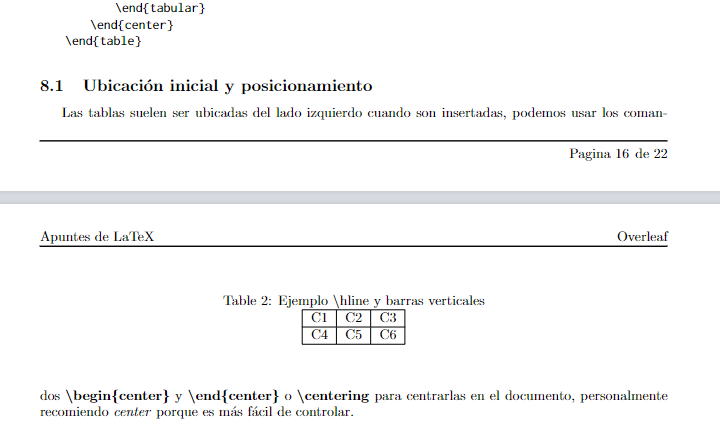
\includegraphics[width=\textwidth]{recursos/tablas_mal pos_2.png}
    \end{center}
\end{figure}

Las tablas que vemos en las imágenes anteriores son las que ya pusimos previamente, pero con un posicionamiento por defecto. Vemos que la Figura \ref{fig: 2} posiciona la tabla al principio de la página 15, previo a la sección de Tablas y tabulación; la Figura \ref{fig: 3} posiciona otra tabla al principio de la siguiente página, no donde nosotros lo deseamos.

Podemos pasar un parámetro de posicionamiento entre corchetes a \LaTeX dónde queremos la tabla, en todas las tablas usadas en este documento se utiliza el parámetro \textit{H}, esto debido a que permite que la tabla se ponga justo a continuación del último objeto o texto donde estuvimos posicionados, respetando el espacio de los objetos o textos a continuación. A continuación se muestra la lista de parámetros de posicionamiento:
\begin{enumerate}
    \item \textbf{h}: pone la tabla aproximadamente aquí.
    \item \textbf{p}: pone la tabla en una página especial, solo para tablas.
    \item \textbf{t}: pone la tabla en la parte superior de la página.
    \item \textbf{b}: pone la tabla en la parte inferior de la página
    \item \textbf{!}: fuerza el posicionamiento de la tabla en base a los parámetros listados aquí.
    \item \textbf{H}: pone la tabla exactamente aquí. Requiere del paquete \textbf{float} para poder ser utilizado.
\end{enumerate}
\begin{lstlisting}
    \begin{document}
        % Parámetro entre corchetes ([]) con el valor H para
        % posicionar estrictamente en dicha posición al
        % objeto.
        \begin{table}[H]
        
        \end{table}
    \end{document}
\end{lstlisting}

\textit{Nota}: personalmente recomiendo el parámetro H, posiciona la tabla donde queremos y respeta el espacio del resto del contenido del documento.

En ocasiones, cuando se está escribiendo un documento y se está trabajando con tablas, estas pueden chocar con el posicionamiento o espacio de las imágenes, por ejemplo, si tenemos una imagen, en seguida una tabla y luego una nueva sección o subsección, en vez de seguir ese orden, puede que ocurra que aparezca la imagen, la sección y luego la tabla, cosa que no va de acuerdo al orden que buscamos, para solucionar eso, puede insertar el comando \textbf{\textbackslash{newpage}} entre el fin de la imagen y el inicio de la tabla para lograr acomodar las cosas.

Otra solución es utilizar el parámetro entre corchetes ([]) con el valor H para las figuras, imágenes o ecuaciones:
\begin{lstlisting}
    \begin{document}
        Imagen
        \begin{figure}[H]
        
        \end{figure}
        Tabla
        \begin{table}[H]
        
        \end{table}
    \end{document}
\end{lstlisting}

De esta manera, ambos objetos respetan su propio posicionamiento y espacio, sin chocar ni afectar al resto de objetos o textos.
\begin{lstlisting}
    \begin{table}[H]
        \begin{center}
            \caption{Ejemplo de tabla con formato APA}
            \label{tab: 4}
            \begin{tabular}{l l l l}
                \hline
                Título 1 & Título 2 & Título 3 & Título4 \\
                \hline
                aaaaaaaaaaa         & bbbbbbbbbbbb  & cccccccc      & lorem impsum \\
                prueba 1            & prueba 2      & prueba tres   & prueba four \\
                texto de relleno    & rellenando    & info adicional& oh yeah \\
                \hline
            \end{tabular}
        \end{center}
    \end{table}
\end{lstlisting}
\begin{table}[H]
    \begin{center}
        \caption{Ejemplo de tabla con formato APA}
        \label{tab: 4}
        \begin{tabular}{l l l l}
            \hline
            Título 1 & Título 2 & Título 3 & Título4 \\
            \hline
            aaaaaaaaaaa         & bbbbbbbbbbbb  & cccccccc      & lorem impsum \\
            prueba 1            & prueba 2      & prueba tres   & prueba four \\
            texto de relleno    & rellenando    & info adicional& oh yeah \\
            \hline
        \end{tabular}
    \end{center}
\end{table}

La Tabla \ref{tab: 4} tiene un formato parecido a lo establecido al formato APA, esto es un ejemplo de como trabajar de forma sencilla con las tablas.


\subsection{Referenciar tablas en el texto}

Para poder referenciar en texto una tabla, es recomendable poner el texto de referencia dentro del comienzo de la tabla y previo del comienzo de \textbf{tabular}, antes de centrarla si es que se quiere centrar, para que, si se mueve la tabla, el texto de referencia se vaya con ella también, ya que si se pone afuera, el texto puede no quedar junto o cerca a la tabla.


\subsection{Ancho fijo de columnas}

Para que una tabla tenga columnas con un ancho fijo, se utiliza el paquete \textbf{array}.
\begin{center}
    \textit{\textbackslash{usepackage\{array\}}}
\end{center}

El tamaño del ancho de columna se indica dentro de llaves en las llaves donde se indica la alineación del contenido de las columnas, se tiene que tener conocimiento sobre las unidades de medida de \LaTeX.
\begin{center}
    \textbackslash{begin\{tabular\}\{m\{5cm\} m \{3cm\} m\{1cm\}\}}
\end{center}

En esta ocasión, como podemos recordar de los parámetros de las tablas convencionales (l, c, r), en este caso dejamos de lado los parámetros de alineación del contenido de columnas y los sustituiremos por los siguientes:
\begin{itemize}
    \item \textbf{m}: alinea el texto en medio de la columna.
    \item \textbf{b}: alinea el texto en la parte inferior de la columna.
    \item \textbf{p}: alinea el texto en la parte superior de la columna.
\end{itemize}
\begin{lstlisting}
    \begin{table}[H]
        \begin{center}
            \caption{Ejemplo de tabla con ancho de columna fijo}
            \label{tab: 5}
            \begin{tabular}{|m{5cm}|m{3cm}|m{1cm}|}
                \hline
                1   & 2 & 3 \\
                4   & 5 & 6 \\
                \hline
            \end{tabular}
        \end{center}
    \end{table}
\end{lstlisting}
\begin{table}[H]
    \begin{center}
        \caption{Ejemplo de tabla con ancho de columna fijo}
        \label{tab: 5}
        \begin{tabular}{|m{5cm}|m{3cm}|m{1cm}|}
            \hline
            1   & 2 & 3 \\
            4   & 5 & 6 \\
            \hline
        \end{tabular}
    \end{center}
\end{table}

La Tabla \ref{tab: 5} tiene ancho de de columna de 5cm, 3cm y 1cm (izquierda a derecha).


\subsection{Combinar filas y columnas}

Se requiere del paquete \textbf{multirow} para poder combinar columnas y filas.
\begin{center}
    \textit{\textbackslash{usepackage\{multirow\}}}
\end{center}

Se debe tener cuidado con los parámetros que reciben los comandos \textbf{\textbackslash{multirow\{\}\{\}\{\}}} y \\ \textbf{\textbackslash{multicolumn\{\}\{\}\{\}}} ya que varían un poco: para ambos, el primer parámetro recibe cuántas columnas o filas se van a combinar y el tercero indica el texto o contenido de dichas filas o columnas combinadas, el segundo parámetro varia dependiendo si se combina filas o columnas, para el primer caso, el parámetro recibe el ancho de fila (utilizando unidades de \LaTeX) y, para el segundo caso, recibe la alineación de las columnas (l, c, r):
\begin{lstlisting}
    \begin{table}[H]
        \begin{center}
            \caption{Ejemplo con tabla con columnas combinadas}
            \label{tab: 6}
            \begin{tabular}{c|c|c}
                \hline
                \multicolumn{3}{c}{3 celdas combinadas} \\
                \hline
                1   & 2 & 3 \\
                4   & 5 & 6 \\
                \hline
            \end{tabular}
        \end{center}
    \end{table}
    
    \begin{table}[H]
        \begin{center}
            \caption{Ejemplo con tabla con filas combinadas}
            \label{tab: 7}
            \begin{tabular}{m{5cm}|m{3cm}|m{1cm}}
                \hline
                1   & 2 & 3 \\
                \hline
                \multirow{2}{5cm}{2 filas combinadas}   & 4 & 5 \\
                &   6 & 7 \\
                \hline
                8   & 9 & 10 \\
                \hline
            \end{tabular}
        \end{center}
    \end{table}
\end{lstlisting}

\textit{Nota}: fijarse bien en como se distribuyen los elementos de cada celda si se desea combinar, ya sea filas o columnas, en el ejemplo anterior, por ejemplo, dependiendo si la tabla tendrá tres columnas, \textit{multicolumn} solo puede tomar como máximo tres columnas a combinar, si tiene cinco filas, \textit{multicolumn} se puede poner en cualquiera de esas cinco columnas.
\begin{table}[H]
    \begin{center}
        \caption{Ejemplo con tabla con filas combinadas}
        \label{tab: 6}
        \begin{tabular}{c|c|c}
            \hline
            \multicolumn{3}{c}{3 celdas combinadas} \\
            \hline
            1   & 2 & 3 \\
            4   & 5 & 6 \\
            \hline
        \end{tabular}
    \end{center}
\end{table}
\begin{table}[H]
    \begin{center}
        \caption{Ejemplo con tabla con columnas combinadas}
        \label{tab: 7}
        \begin{tabular}{m{5cm}|m{3cm}|m{1cm}}
            \hline
            1   & 2 & 3 \\
            \hline
            \multirow{2}{5cm}{2 filas combinadas}   & 4 & 5 \\
            &   6 & 7 \\
            \hline
            8   & 9 & 10 \\
            \hline
        \end{tabular}
    \end{center}
\end{table}

Repetimos, se debe tener cuidado combinando filas y columnas, para el primer caso, y con un ancho de columna fijo, el ancho de la columna donde se combinarán filas debe coincidir, tanto en la tabla, como en el comando \textbf{multirow} (\textit{Tabla \ref{tab: 6}}), y el número de columnas a combinar debe coincidir con el número real de columnas en una tabla con \textbf{multicolumn} (\textit{Tabla \ref{tab: 7}}).
